%!TEX root] ../report.tex

\section{Trainingsmodelle}

Generell:
\begin{description}
    \item[kurzfristig] Leistungsveränderungen durch optimale Gestaltung der Einzelreize anstoßen
    \item [mittelfristig] Leistungsfähigkeit steigern und herausbilden der optimalen Form für einen bestimmten Zeitraum
    \item [langfristig] Leistungspotential langfristig ausschöpfen
\end{description}

\subsection{kurzfristig}

Grundlegende Begriffe:
\begin{description}
    \item [Homöostase] dauerhaft aufrechthaltbarer Gleichgewichtszustand in Ruhe
    \item [Heterostase] Störung der Homöostase
    \item [Belastung] objektiv von Außen auf den Organismus wirkende Faktoren Umstellung] Zustandsveränderung der Funktionssysteme im Rahmen ihres Regulationsbereiches durch Belastung (auch Aktivierung)
    \item [Beanspruchung] individuelle Reaktion des Organismus auf eine Belastung
    \item [(Max) Steady State] zeitlich begrenzt aufrechthaltbare (maximale) Leistung während der Belastung
    \item [Ermüdung] reversible Leistungsminderung durch Beanspruchung
    \item [Regeneration] Prozesse zur Wiederherstellung der Homöostase
    \item [Superkompensation] überschießende Wiederherstellung der Leistungsfähigkeit
    \item [Adaptation] zeitlich stabile, reversible Steigerung der Leistungsfähigkeit durch Beanspruchung
    \item [Deadaptation] Rückbildung der Leistungsfähigkeit durch fehlende Beanspruchung
\end{description}

Zeitlicher Ablauf:

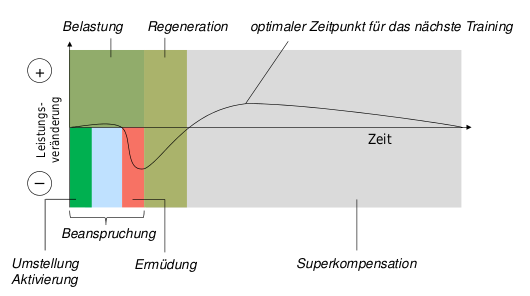
\includegraphics[width=\textwidth]{pictures/zeitlicher_ablauf}

\begin{minipage}{0.6\textwidth}
Beanspruchung:
\begin{itemize}
    \item beanspruchte Systeme: Herz-Kreislauf-System, Atmung, Stoffwechsel, Hormonsystem, Nervensystem)
    \item Einflussfaktoren auf Beanspruchung: Leistungsfähigkeit, Ermüdungszustand, Erkrankungen, Schmerzen, Umweltbedingungen, psychischer Zustand, Motivation
    \item Höhere Leistungsfähigkeit führt bei gleicher Belastung zu einer geringeren Beanspruchung und geringerer Ermüdung. Außerdem ermöglicht sie höhere Belastungen und eine schnellere Regeneration.
\end{itemize}
Ermüdung:
\begin{itemize}
    \item Ursachen: Anhäufung von Stoffwechselendprodukten, Entleerung der Energiedepots, Störung der peripheren Informationsübertragung, Zentralnervöse Ermüdung
\end{itemize}
\end{minipage}
\begin{minipage}{0.4\textwidth}
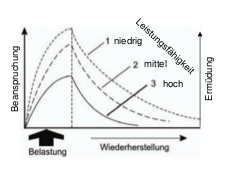
\includegraphics[width=\textwidth]{pictures/bs1}
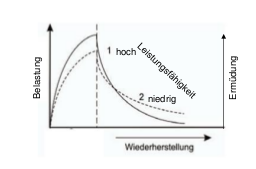
\includegraphics[width=\textwidth]{pictures/bs2}
\end{minipage}

\begin{itemize}
    \item Auswirkungen: Kraft- \& Schnelligkeitsverlust, verlängerte Reaktionszeiten, verminderte Genauigkeit, verminderte Konzentrationsfähigkeit
    \item  Toleranzbereich in dem Ermüdung ``zurückgedrängt'' werden kann
    \item insgesamt eher schlecht verstandenes Phänomen
\end{itemize}

Regenerationszeit physiologischer Systeme und Wirksamer Belastungsreiz:

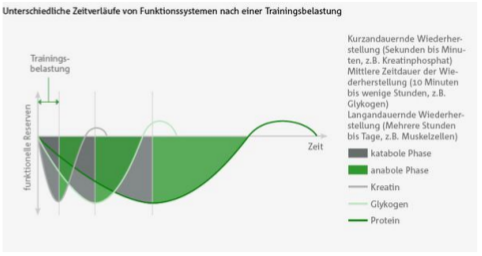
\includegraphics[width=0.5\textwidth]{pictures/regenerationszeit}
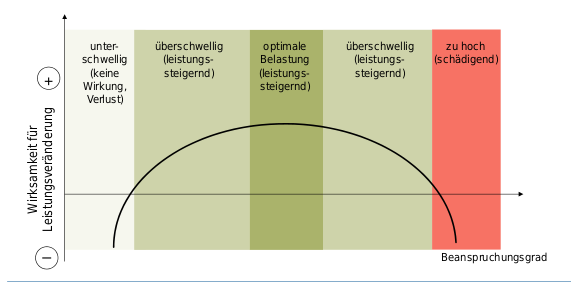
\includegraphics[width=0.5\textwidth]{pictures/belastungsreiz}

\subsection{mittelfristig}

Adaptionen durch richtige Trainingsabstände:
\begin{itemize}
    \item Herz-Kreislauf-System (Herzvergrößerung, Ruheherzschlagfrequenz)
    \item Sauerstoffaufnahme (Hämoglobin, Kapillarisierung)
    \item Energiespeicher (Phosphatspeicher, Glykogenspeicher)
    \item Energiegewinnung (Phosphat-, Kohlenhydrat-, Fettstoffwechsel)
    \item Muskeln (Faserverteilung, Hypertrophie)
    \item Neuromuskuläres System (Sensomotorik, Propriorezeption)
    \item Immunsystem, Hormonsystem
    \item Reorganisation von neuronalen Strukturen (Wahrnehmungs-, Entscheidungsvorgänge, Bewegungskontrolle)
\end{itemize}

\begin{minipage}{0.5\textwidth}
Bei zu großen Trainingsabständen folgt Stagnation, ebenso wie durch den Deckeneffekt. Bei Ausbleiben eines Trainingsreizes kommt es zur Deadaption zur Baseline. Zu kleine Trainingsabstände können auch zu einem Leistungsverlust führen.

Overreaching und Overtraining:
\begin{description}
    \item [Overloading] kurzzeitige, bewusste Überforderung
    \item [Overreaching] bei Entlastung nach ca. 2 Wochen vollständige Regeneration mit Superkompensationseffekt
    \item [Overtraining] chronische Überforderung,  anhaltender pathologisch Zustand, reduzierte körperliche Leistungsfähigkeit, nur durch lange Pause zu bewältigen
\end{description}

Indikatoren für Overtraining:
\begin{itemize}
    \item Blutwerte: Muskelglykogen, reatinkinase, Adrenalin, Noradrenalin, Ammoniak
\end{itemize}
\end{minipage}
\begin{minipage}{0.5\textwidth}
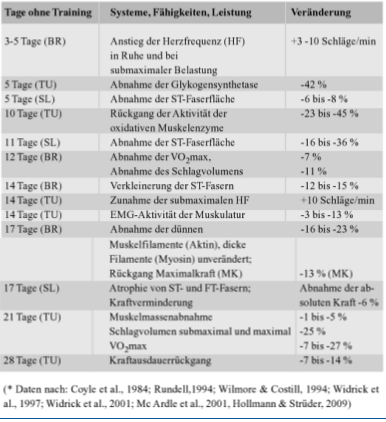
\includegraphics[width=\textwidth]{pictures/leistungsverlust_umfang}
\end{minipage}

\begin{itemize}
    \item Ruhepuls (Messung morgens direkt nach dem Aufwachen). Erhöhte Pulswerte $\rightarrow$ evtl. Übertraining. Kontinuierliche Absenkung $\rightarrow$ Anpassungssignal
    \item Zittern, erhöhte Körpertemperatur
    \item psychischer Zustand: Unlust, Schlafstörungen, Apathie, Depressionen
\end{itemize}

Periodisierung ist die phasenförmige Veränderung von Teilzielen, Belastungen, Methoden und Organisationsformen zur Herausbildung der optimalen Form für einen bestimmten Zeitraum. Man periodisiert zur Vermeidung von Deckeneffekten, Übertraining und Motivationsproblemen. Außerdem kann man den Superkompensationseffekt und eine temporäre Stabilität der Fähigkeiten ausnutzen.

Trainingsperioden:
\begin{description}
    \item[Vorbereitungsperiode] allgemeine konditionelle Vorbereitung. Umfang hoch, Intensität mittel-hoch
    \item[Wettkampfperiode] Entwicklung und Stabilisierung der Höchstform. Umfang gering, Intensität hoch, ausreichend Regeneration
    \item [Übergangsperiode] aktive Erholung. Umfang niedrig, Intensität niedrig
    \item [Makrozyklus] uneinheitlich 3 Monate bis ein Jahr
    \item [Mesozyklus] uneinheitlich 2 Wochen bis 3 Monate, unterschiedliche Schwerpunkte
    \item [Mikrozyklus] dauer idR eine Woche
\end{description}

Je nach Bedürfnissen kann man nicht nur Einfachperiodisieren (ein überragender Wettkampfhöhepunkt), sondern aucch doppel- oder dreifachperiodisierung vornehmen.

Zyklen:
\begin{description}
    \item[Aufbauzyklus] Entwicklung einzelner konditioneller Fähigkeiten. Faustregeln:
    \begin{itemize}
        \item Stabiler Leistungsgewinn nach  ca. 6 Wochen
        \item auf 3 Belastungs-MIZ erfolgt ein Entlastungs-MIZ
    \end{itemize}
    \item [Taperzyklus] Vorbereitung auf Höchstleistung
    \begin{itemize}
        \item Reduktion des Trainingsumfangs zum Zwecke der Leistungsmaximierung
        \item Beseitigen der trainingsbedingten Ermüdung, Aufladen der Energiespeicher $\rightarrow$ Reduktion des Trainingsumfangs
        \item Vermeidung des Abklingens der positiven Trainingsadaptionen $\rightarrow$ Beibehalten der Trainingsintensität
        \item Reduktion kann schrittweise, linear oder exponentiell erfolgen
    \end{itemize}
\end{description}

\begin{minipage}{0.65\textwidth}
\begin{description}
\item
    \begin{itemize}
        \item Erfahrungswerte: Phase der unmittelbaren Wettkampfvorbereitung ca. 6-7 Wochen, Umfangsmaximum 2-3 Wochen vor Wettkampf, Intensitätmaximum 1-2 Wochen vor Wettkampf. Dabei Umfang von allgemeinen Trainingsinhalten früher reduzieren als von speziellen.
    \end{itemize}
    \item [Wettkampfzyklus] Erreichen und Halten der Höchstleistung
    \item [Regenerationszyklus] Regeneration
\end{description}

Unterstützung durch Höhentraining:
\begin{itemize}
    \item Effekte: Erhöhung der EPO-Ausschüttung, Zunahme rote Blutkörperchen und Hämoglobin, Verbesserte Kapillarisierung
    \item Varianten: Training und Schlaf in der Höhe (klassisch), nur jeweils eins oben oder Simulation von Höhentraining
    \item Empfohlene Parameter: Mindestens 3 Wochen (3-6 Tage Akklimatisierung, 14 Tage Training, 2-5 Tage Erholung), Höhe 1800-2800m, dabei erhöten Wasser, Kohlenhdrat und Eisenbedarf beachten
    \item Wirkung der klassischen Variante gut abgesichert (Effekt hält 2-3 Wochen an)
\end{itemize}
\end{minipage}
\begin{minipage}{0.35\textwidth}
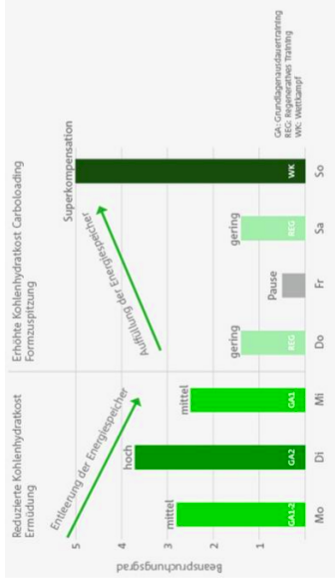
\includegraphics[width=\textwidth]{pictures/carbo_loading}

Unterstützung durch Carbo-Loading
\end{minipage}

\subsection{langfristig}

\begin{itemize}
    \item Modellvorstellung über den Aufbau von Leistungsfähigkeit und –bereitschaft von den sportlichen Anfängen bis zur internationalen Höchstleistung
    \item Gesamtdauer ca. 10 Jahre, d.h. ca. 2 Jahre pro Stufe
    \item Konkrete Zielstellung: Erfüllung der Aufgaben jeder Etappe. Nicht: Höchstleistung in der jeweiligen Altersklasse
    \item Die potentielle Leistungsfähigkeit steigt bis zum Höchstleistungsalter. Dabei ist es wichtig die Leistungsreserven nicht zu früh auszuschöpfen.
    \item Quantitätsgesetz: Je höher das Leistungsniveau, desto mehr Trainingsaufwand ist erforderlich
    \item Qualitätsgesetz: Je höher das Leistungsniveau, desto spezifischer müssen die Leistungskomponenten trainiert werden
    \item mit höherem Alter wird das Training zunehmend spezialisierter.
\end{itemize}

\subsubsection{Zusammenfassung}

Trainingsprinzipien:
\begin{description}
    \item[kurzfristig] Prinzip des wirksamen Belastungsreizes, der individualisierten Belastung und der optimalen Relation von Belastung und Erholung
    \item [mittelfristig] Prinzip der Wiederholung und Dauerhaftigkeit, der  zeitlichen Strukturierung und der variierenden Belastung
    \item [langfristig] Prinzip der progressiven Belastungssteigerung, des langfristigen Leistungsaufbaus und der zunehmenden Spezialisierung
\end{description}

Fazit: Pro-Argumente:
\begin{itemize}
    \item Best-Practice-Lösungen der Praxis
    \item Veranschaulichung von Phänomenen/Problemen
    \item teilweise Entsprechungen auf molekularer Ebene (z.B. aus Glycogen- und Enzym-Stoffwechsel; Jakowlew, 1955)
\end{itemize}

Fazit: Contra-Argumente
\begin{itemize}
    \item Verallgemeinerung unzulässig (Superkompensation im Labor nur für einige physiologische Parameter nachgewiesen)
    \item Gültigkeit auf Individualebene zweifelhaft?
    \item Wechselwirkung verschiedener Trainingsreize werden nicht berücksichtigt
    \item Angabe präziser Indikatoren oder Zeitangaben nicht möglich (?)
    \item Kurzfristige und mittelfristige Modelle gelten primär für Ausdauer \& Kraftleistungen - keine Gültigkeit für nformationsverarbeitung
\end{itemize}

Insgesamt ist individualisierte Trainingssteuerung notwendig.
